\section{Durchführung}
\label{sec:Durchführung}
In der Durchführung des Versuches wurde zuerst das Entladeverhalten eines RC-Kreises untersucht, um die Zeitkonstante des Stromkreises zu bestimmen. Dafür wurde die Schaltung aus \autoref{fig:aufbau1} aufgebaut. Dabei wurde für den Rechteckgenerator ein Funktionengenerator angeschlossen, der auf ein Rechtecksignal gestellt wurde. Die Einstellungen am Funktionengenerator wurden dabei so gewählt, dass die gemessene Spannung $U_C$ auf etwa ein Zehntel ihres Ausgangswertes fällt. Mit diesem Versuchsaufbau konnte dann eine Entladekurve auf dem Oszilloskop dargestellt werden aus der die Messwerte zur Bestimmung der Zeitkonstanten ermittelt wurden. \newline
\begin{figure}
    \centering
    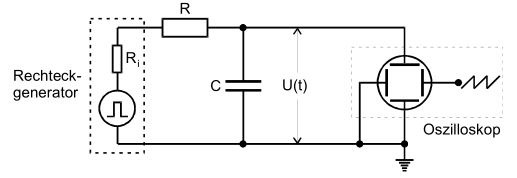
\includegraphics{images/SchaltungZeitkonstante.jpg}
    \caption{Schaltung zur Bestimmung der Zeitkonstanten \cite{VA}}
    \label{fig:aufbau1}
\end{figure}
In der nächsten Messung sollte die Amplitude der Kondensatorspannung eines RC-Gliedes, das an einer Sinusspannung angeschlossen ist, in Abhängigkeit von der Frequenz bestimmt werden. Für die Bestimmung der Messdaten wurde, die in \autoref{fig:aufbau2} dargestellte Schaltung verwendet. Da die Kondensatorspannungsamplitude in Abhängigkeit von der Frequenz über 3 Zehnerpotenzen hinweg gemessen werden sollte, wurden für die Messung Frequenzen zwischen $420 Hz$ und circa $80 kHz$ verwendet.\newline

\begin{figure}
    \centering
    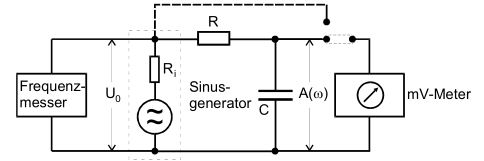
\includegraphics{images/SchaltungFrequenz.JPG}
    \caption{Schaltung zur Untersuchung der Kondensatorspannungsamplitude abhängig von der Frequenz \cite{VA}}
    \label{fig:aufbau2}
\end{figure}
Für die Messreihe zur Bestimmung der Phasenverschiebung zwischen Generator- und Kondensatorspannung wurde eine Schaltung nach \autoref{fig:aufbau3} verwendet. Dafür wurde die Kondensatorspannung $U_C$ auf einen Eingang des 
Zweikanaloszilloskops gegeben und die Generatorspannung $U_G$ auf den anderen Eingang. Als Messwerte wurden einerseits die zeitlichen Abstände der Nulldurchgänge beider Spannungen und andererseits die Gesamtschwingungsdauer jeweils für unterschiedliche Frequenzen notiert. \newline
\begin{figure}
    \centering
    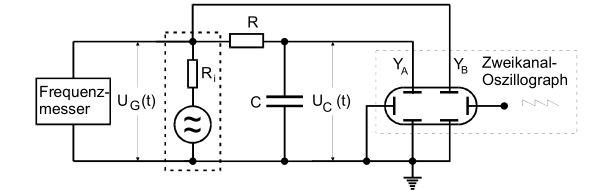
\includegraphics{images/SchaltungPhaVersch.JPG}
    \caption{Schaltung für die Bestimmung der Phasenverschiebung zwischen Generator- und Kondensatorspannung \cite{VA}}
    \label{fig:aufbau3}
\end{figure}
Im letzten Versuchsteil sollte die Funktion des RC-Kreises als Integrator gezeigt werden. Dafür wurde erneut die Schaltung aus \autoref{fig:aufbau3} genutzt. Die Frequenz wurde so eingestellt, dass man den Verlauf der Generator- und der Kondensatorspannung gut auf dem Bildschirm des Oszilloskops erkennen konnte. Es wurden dann nacheinander eine Rechteck-, Dreiecks- und Sinusspannung auf das RC-Glied gegeben und jeweils Fotos von den entstandenen Spannungskurven auf dem Oszilloskopbildschirm gemacht.